% -------------------------------------------------------------------------------------------------
% Definitionen
% -------------------------------------------------------------------------------------------------
\documentclass[
    fontsize=12pt,                      % Schriftgröße 12 pt
    paper=a4,                           % Seitengröße A4
    twoside=off,                       % zweiseitiger Druck
    DIV=15,                             % Seiteneinteilung
    BCOR=12mm,                          % Bindekorrektur
    headings=normal,                    % normal große Überschriften
    headsepline=false,                   % Trennlinie unter der Kopfzeile
    footsepline=false,                  % Trennlinie über der Fußzeile
    headinclude=true,                   % Kopfzeile zählt zum Textkörper
    footinclude=false,                  % Fußzeile zählt nicht zum Textkörper
    toc=listof,                         % Verzeichnisse der Gleitumgebungen ins Inhaltsverzeichnis
    toc=bib,                            % Literaturverzeichnis ins Inhaltsverzeichnis
    chapterprefix=false,                % vor Kapitelnummern steht "Kapitel"
    appendixprefix=false,               % vor Anhangüberschriften steht "Anhang"
    numbers=noendperiod,                % Keinen Punkt hinter die letzte Zahl eines Kapitels (auch bei Anhang)
    captions=tableabove,                % Tabellenüberschriften setzen
    footnotes=multiple,                 % Erkennung von mehreren Fußnoten hintereinander
    bibliography=oldstyle,              % Literaturverzeichnis: openstyle oder oldstyle
    draft=false,                        % Entwurfsstadium
]{scrreprt}


% Paket Includes
% ----------------------------
\usepackage[T1]{fontenc}                % deutsche Umlaute und Sonderzeichen
\usepackage[utf8]{inputenc}             % Umlaute koennen direkt im Quelltext stehen
\usepackage[ngerman]{babel}             % neue deutsche Rechtschreibung 
\usepackage{lmodern}
\usepackage{graphicx}                   % Bilder einfügen
\usepackage{tabularx}                   % Tabellen mit fester Breite und variabler Spaltenbreite
\usepackage{array,longtable}            % Tabellen mit Seitenumbruch
\usepackage{booktabs}                   % bessere horizontale Linien in Tabellen
\usepackage{array,ragged2e}             % mehr Spaltentypen in Tabellen und neue Spaltentypen
\usepackage{dcolumn}                    % Spalten am Dezimaltrenner ausrichten
\usepackage{amsmath}
\usepackage[                            % Unterabbildungen mit folgenden Parametern:
            font=footnotesize,          % kleine Schrift
            labelfont={sf,bf},          % Labels fett und serifenlos
            textfont={sf},              % Text serifenlos
            format=hang,                % hängender Einzug
           ]{caption}
\usepackage{float}      
\usepackage{hyperref}                   % URL links     
\usepackage{xcolor} 
\usepackage{listings}
\usepackage{subfig}

\definecolor{myblue}{rgb}{0,0.3137,0.5843}
\definecolor{mygreen}{rgb}{0,0.6,0}
\definecolor{myred}{rgb}{0.7529,0.3137,0.3019}

\newcommand{\Farbcode}[1]{\texttt{\textbf{\textcolor{myred}{#1}}}}


% Kopf- und Fußzeile
% ----------------------------
\usepackage{scrlayer-scrpage} 
\setkomafont{pagehead}{\sffamily\small}
\setkomafont{pagefoot}{\sffamily\small}
%\automark{chapter}
\lohead{Modul Embedded Systems 2 – Steuergeräte, Vernetzung, Software} \cohead{} \rohead{Übung 1-4}
\lofoot{\includegraphics[height=10pt]{Figures/HSMW-Logo-klein} HS Mittweida, INW, Prof. Thomanek}
\cofoot{} \rofoot{\thepage}

\pagestyle{headings}
\renewcommand*{\chapterpagestyle}{headings}% Nicht zu empfehlen, aber du willst das offenbar trotzdem.


\setcounter{secnumdepth} {3}
\addto\captionsngerman{\renewcommand{\figurename}{Abb.}}    % Verwende Abb. x.x anstatt Abbildung x.x
\renewcommand{\thefigure}{\arabic{figure}}
% -------------------------------------------------------------------------------------------------
% Dokument
% -------------------------------------------------------------------------------------------------

\begin{document}


\chapter*{Übung 1-4 -- Übermitteln von CAN-Daten}

Über einen \text{Thermistor} (Heißleiter, NTC (MF52-103 3435)) soll die Temperatur gemessen werden. Dabei wird der Spannungsabfall über den temperaturabhängigen Widerstand mithilfe eines Spannungsteilers gemessen.

\vskip 0.2cm
\noindent

Die gemessene Temperatur soll auf dem \textbf{CAN übertragen} werden. Dafür wird der Mikrokontroller \textbf{Aurix TC374} verwendet, der eine integrierte CAN-Schnittstelle bietet. Der \textbf{CAN-Transceiver „TLE9251VSJ“} von Infineon ist auf dem TC375 verbaut.

\vskip 0.2cm
\noindent

% Die Kommunikation mit dem CAN-Bus erfolgt über den Anschluss an die Pins CAN-H und CAN-L des Mikrokontrollers, wie in der Abbildung dargestellt.

\vskip 0.5cm
\section*{Schaltungsaufbau} 
\begin{itemize}
\item Spannungsteiler: Vorwiderstand (10~k$\Omega$) an 5V und NTC (10~k$\Omega$ bei $25^\circ$C) an Masse
\item Spannungsabgriff an Eingang P40.9 des Aurix TC375 mit einer Auflösung des ADC von 10~Bit bei Spannungsbereich von 0 \dots 5V
\end{itemize}

\begin{figure}[H]
  \centering
  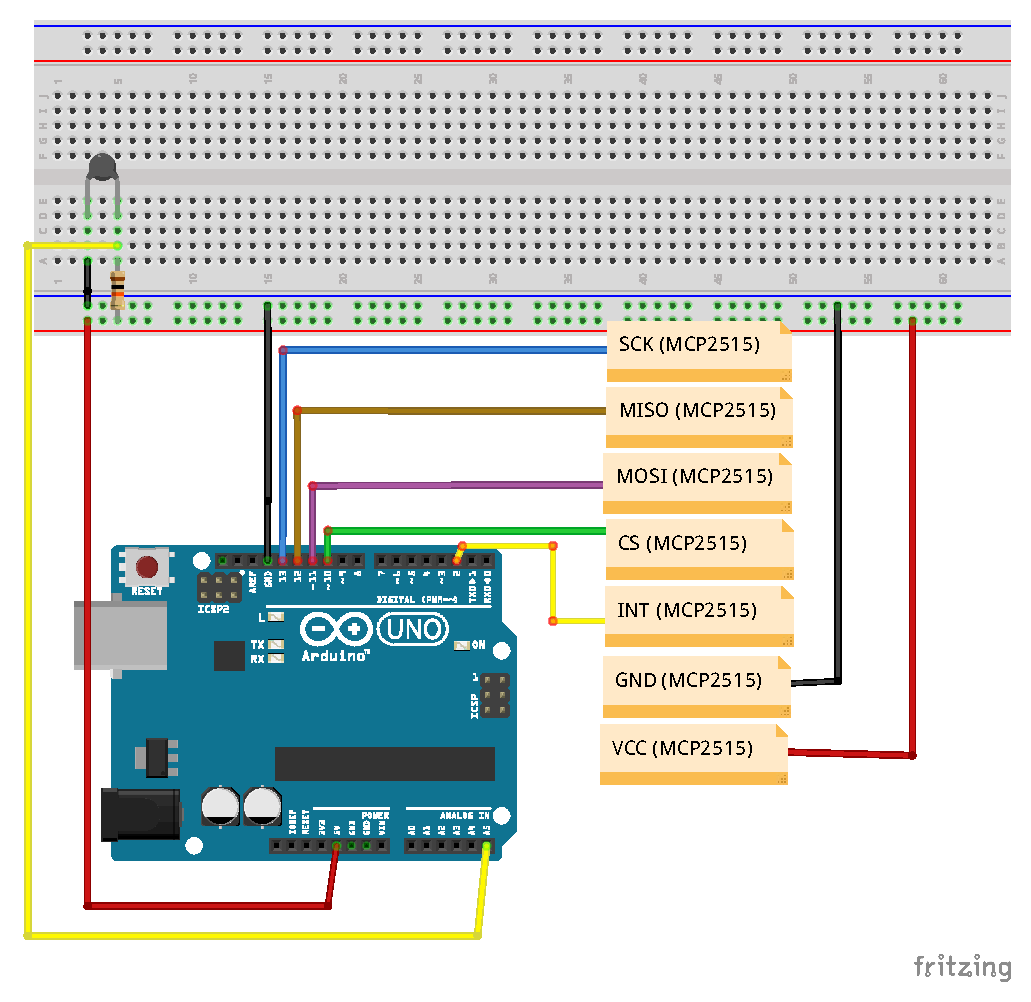
\includegraphics[width=0.55\linewidth]{Fritzing/Uebung_104_Steckplatine.pdf}
  \caption{Steckplatine}%
\end{figure}

\begin{figure}[H]
  \centering
  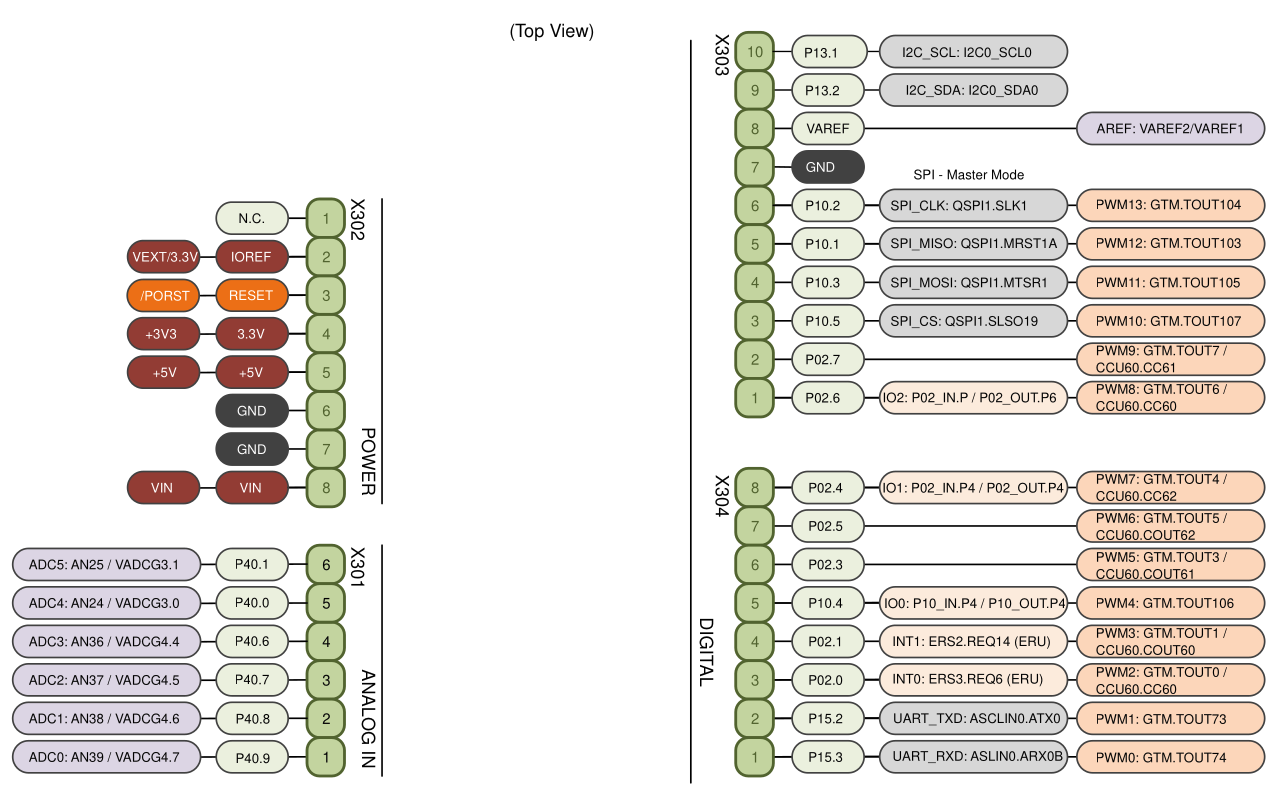
\includegraphics[width=0.90\linewidth]{Figures/Uebung_104_Arduino_Pins.png}
  \caption{Schaltplan Mapping of Arduino Functions to AURIX™ Pin Functions}
\end{figure}
 
\section*{Softwareerstellung} 

Verwenden Sie als Basis das Aurix-Development-Studio-Template \Farbcode{Uebung\_104\_Template.zip}. Importieren sie das Projekt. 

File > Import > General > Existing Projects into Workspace > Select archive file > Browse > Finish

\begin{figure}[H]
  \centering
  \subfloat[][]{
    \raisebox{0.5\height}{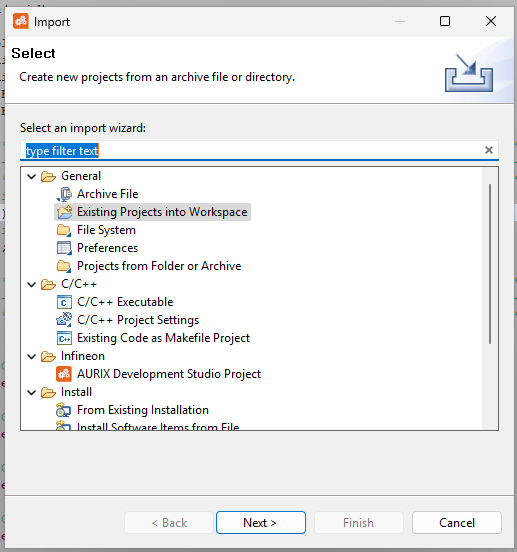
\includegraphics[width=0.45\linewidth]{Figures/Import_1.png}}
  }%
  \quad
  \subfloat[][]{
    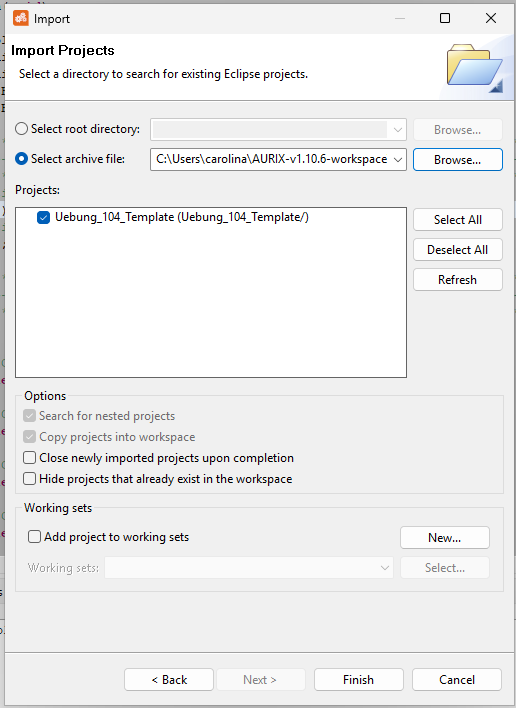
\includegraphics[width=0.45\linewidth]{Figures/Import_2.png}
  }%
  \caption{Importieren eines Projektes in Aurix Studio}%
\end{figure}

Bearbeiten sie die Datei namens \Farbcode{Cpu0\_Main.c}.

\vskip 0.2cm

\noindent
\textbf{Initialisierung:} ( \Farbcode{void core0\_main(void)} )

\begin{enumerate}

%\textbf{Beachte:} Der CAN-ID lautet 100h + <Testplatznummer> -- Somit sendet bspw. der Testplatz 4 seine Temperatur unter der CAN-ID \texttt{\textbf{104h}} und der Testplatz 10 mit der ID \texttt{\textbf{10Ah}}
\item Initialisierung des CAN-Controllers mittels \Farbcode{initMCMCAN()}
\item Initialisierung des EVADC-Modul mittels \Farbcode{initEVADC()}
%\item Setzen der Bitrate auf 500~kBit/s und Taktfrequenz 8~MHz mittels \\ \Farbcode{mcp2515.setBitrate(...)}
%\item Aktivieren des Normal-Modes mittels \Farbcode{mcp2515.setNormalMode()}
%\item Serielle Konsole für Debug-Zwecke aktivieren mittels \Farbcode{Serial.begin(9600)}
\end{enumerate}

\noindent
\textbf{Endlosschleife:} ( \Farbcode{while(1)} )
\begin{enumerate}
\item Temperatur des Thermistors in Kelvin berechnen
\item Spannungswert am Pin A39 mittels \Farbcode{readEVADC()} einlesen.
\item Gemessene Spannung berechnen
\item Widerstand des Thermistors anhand Spannungsteilerregel bestimmen
\item Temperatur aus Widerstandswert bestimmen gemäß Formel
\begin{equation*}
T(R)=\frac{1}{\frac{1}{B}\ln(\frac{R}{R_{25}})+\frac{1}{T_{25}}} 
\end{equation*}
wobei $B$ -- Sensorkonstante, $R_{25}$ -- Widerstand des Thermistors bei $25^\circ$C, $T_{25}$ -- Temperatur in Kelvin ($25^\circ$C)

Ermitteln Sie die Sensorkonstante (B-Wert) aus dem Datenblatt des Thermistors (Siehe OPAL).
\item Ausgeben des Temperaturwert auf einer CAN-Botschaft mittels \\ \Farbcode{transmitCanMessage(unsigned int message, uint32 messageId)}\\
\textbf{Beachte:} Der CAN-ID lautet 100h + <Testplatznummer> -- Somit sendet bspw. der Testplatz 4 seine Temperatur unter der CAN-ID \texttt{\textbf{104h}} und der Testplatz 10 mit der ID \texttt{\textbf{10Ah}}


\item Die Übertragung der Temperatur soll zyklisch aller 1000 ms erfolgen
\end{enumerate}

%\newpage
%\section*{Anhang} 
%\noindent
%\textbf{Arduino-Pins:} (siehe  \Farbcode{can.h})
%\textbf{EVADC Channel and Group} (siehe  \Farbcode{can.h})
\end{document}


